\documentclass[cs4size,a4paper,nofonts]{ctexart}
\usepackage[utf8]{inputenc}
\def\tjf{{\tt{田劲锋}}}
\def\titlec{猜数字游戏}
\def\titlee{Standardized Examination System}
\usepackage[top=2.5cm,bottom=2.5cm,left=3.1cm,right=3.1cm]{geometry} % 页面设置
\usepackage[unicode,breaklinks=true,
colorlinks=true,linkcolor=black,anchorcolor=black,citecolor=black,urlcolor=black,
pdftitle={\titlec},pdfauthor={\tjf},pdfsubject={\titlee}]{hyperref}
\usepackage{tikz} % 画图
\usetikzlibrary{shapes,arrows}
\usepackage{multicol} % 分栏
\usepackage{multirow} % 跨行
\usepackage{longtable} % 长表格
\usepackage{tabularx} % 变宽表格
\usepackage{booktabs} % 表格画线
\usepackage{graphicx} % 图形
\usepackage{color} % 颜色
\usepackage{xcolor} % 颜色
\usepackage{wallpaper} % 背景图片
\usepackage{listings} % 排版代码
\usepackage{verbatim} % 排版代码
\usepackage{url} % 排版链接
\usepackage{shortvrb}
\usepackage{uml} % 画 UML
\usepackage{smartdiagram} % 智能画图
\usepackage{nameref}
\usepackage{rotating} % 横排大图
\usepackage{caption}
\captionsetup{font={small}} % 标题字体大小
\usepackage[inline]{enumitem} % 调整列表样式
\usepackage{paralist} % 排序列表环境

\usepackage{tikz}
\usetikzlibrary{arrows,shadows} % for pgf-umlsd
\usepackage[underline=true,rounded corners=false]{pgf-umlsd}
\usepackage{tikz-uml}

\setmainfont{Times New Roman}
\setCJKmainfont[BoldFont={SimHei},ItalicFont={STFangsong}]{SimSun}  % 主要字体:宋体、黑体
\setCJKsansfont[BoldFont={STZhongsong}]{STFangsong} % 次要字体:仿宋、中宋
\setCJKmonofont{KFKai} % 等宽字体:楷体
\setCJKfamilyfont{liti}{隶书} \newcommand{\liti}{\CJKfamily{liti}}

\CJKsetecglue{\hspace{0.1em}}
\renewcommand\CJKglue{\hskip -0.3pt plus 0.08\baselineskip}
\frenchspacing
\widowpenalty=10000
\linespread{1.5} % 1.5 倍行距
\setlength{\parskip}{2pt plus 2pt}
\renewcommand{\baselinestretch}{1.5}

% \setlength{\abovecaptionskip}{1pt}
% \setlength{\belowcaptionskip}{0pt}
\setlength{\intextsep}{8pt}
\setlist{topsep=0pt,partopsep=0pt,itemsep=0pt,parsep=0pt}
%\setlist[enumerate,1]{label=(\Alph*)}

\makeindex
\pagestyle{plain}

\begin{document}
\newcommand{\tabincell}[2]{\begin{tabular}{@{}#1@{}}#2\end{tabular}}
\newcommand{\tabincelll}[3]{\begin{tabular*}{#1}{@{}#2@{}}#3\end{tabular*}}
\renewcommand{\tabularxcolumn}[1]{m{#1}}
\newcommand{\vil}{\,\vline \hspace{.5em} }


\newcommand{\des}[2]{\makebox[2em][s]{\bf #1}\quad #2}
\newcommand{\function}[5]{\CTEXnoindent\vspace{1em}\par
\begin{minipage}{\textwidth}
    \underline{\makebox[\textwidth][l]{\it{#1}}}\\
    {\tt {{#3}} {\bfseries #1}(#2);}\\
    \des{返回}{#4}\\
    \des{描述}{#5}
\end{minipage}\par
\CTEXindent}

\newcommand\pictext{\linespread{1}\centering}

\lstset{language=C++,
  numbers=left,
  keywordstyle=\bfseries,
  frame=tb,
  morekeywords=[1]{perror,assert,printf,fprintf,scanf,sscanf},
  morekeywords=[2]{},
}


%%%% 开始 %%%%
\begin{titlepage}

\begin{center}


\includegraphics[height=1cm]{image/haut.png}

\vspace*{1cm}
{\liti\fontsize{48pt}{50pt}{课\quad 程\quad 设\quad 计}}

\vspace*{4cm}
{\fontsize{36}{80}\sf\bfseries \titlec}

\vspace*{1cm}
{\fontsize{30}{70}\sf\bfseries \titlee}

\vfill
{\large
\newcommand{\ctline}[2]{\makebox[6em][s]{\bf #1}:\underline{\makebox[14em][c]{\qquad #2\qquad}}\\}
\ctline{课程设计名称}{数据结构课程设计}
\ctline{专业班级}{计算机 1303 班}
\ctline{学生姓名}{\tjf}
\ctline{学号}{201316920311}
\ctline{指导教师}{白\quad 浩}
\ctline{课程设计时间}{\today}
}

\end{center}

\end{titlepage}


{\linespread{1}
\tableofcontents
\vfill\centering
%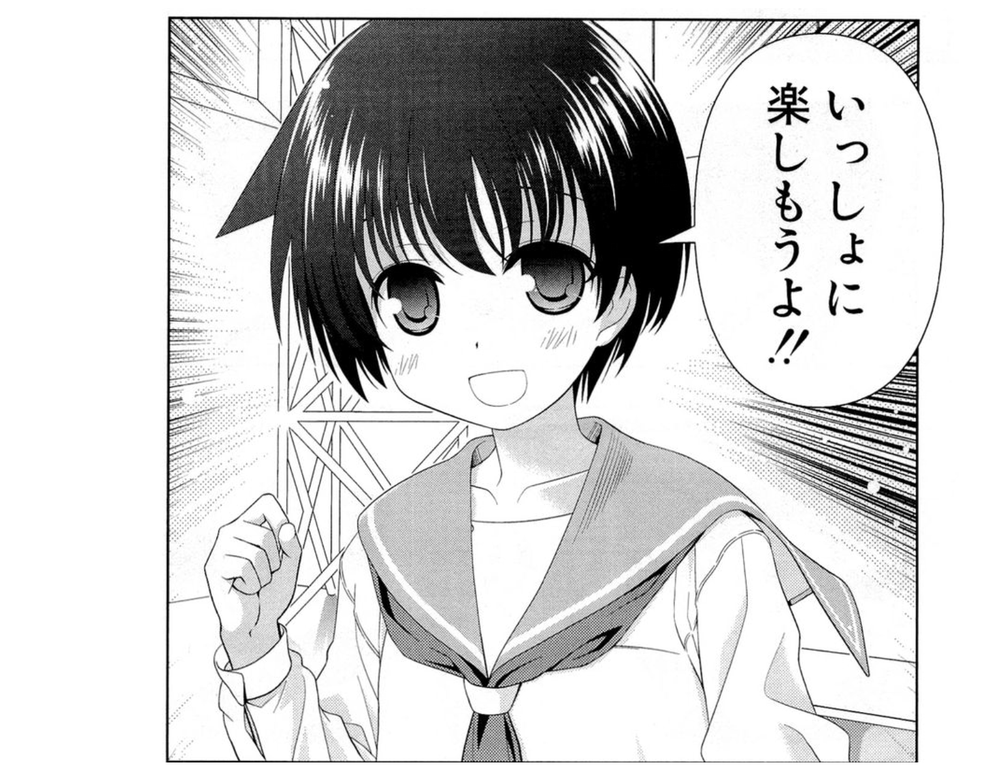
\includegraphics[height=5cm]{image/saki.png}
\vfill}\newpage

\section*{\underline{~软件工程~}专业课程设计任务书}
% \addcontentsline{toc}{section}{课程设计任务书}
% \ThisCenterWallPaper{1}{source/task.pdf}
\begin{center}

\begin{tabular}{|c|c|}\hline
{\bf 学生姓名} & \makebox[5em][c]{\tjf} \vil
\makebox[4em][c]{\bf 专业班级} \vil
\quad 软件 1305 班 \quad \vil
\makebox[4em][c]{\bf 学~号} \vil
201316920311 \\\hline
{\bf 题~目} & \quad \titlec \\\hline
{\bf 课题性质} & \makebox[12em][c]{其他} \vil
{\bf 课题来源} \vil \makebox[11em][c]{自拟课题} \\\hline
{\bf 指导教师} & \makebox[12em][c]{刘扬} \vil
{\bf 同组姓名} \vil \makebox[11em][c]{无} \\\hline
{\bf 主要内容} & {\begin{minipage}[c][5cm][c]{12cm}
操作系统是控制应用程序执行的程序,并充当应用程序和计算机硬件之间的接口。一个操作系统的主要功能有:
\begin{enumerate}
\item 处理器管理
\item 存储器管理
\item 设备管理
\item 文件管理
\end{enumerate}
现在的桌面操作系统多是多任务分时操作系统。
\end{minipage}} \\\hline
{\bf 任务要求} & {\begin{minipage}[c][5cm][c]{12cm}
目标是完成一个基本可用的图形界面操作系统,包括如下基本模块:
\begin{enumerate}
\item 进程:中断处理、多任务调度、系统保护
\item 存储管理:内存分配、进程空间管理
\item I/O 系统:鼠标、键盘和屏幕的控制
\item 文件系统:文件与可执行程序的读取和加载
\end{enumerate}

系统提供命令行用户接口和图形化用户接口,允许使用 C 语言编写系统应用程序,可以从 FAT12 格式软盘启动。
\end{minipage}} \\\hline
{\bf 参考文献} & {\begin{minipage}[c][5cm][c]{12cm}
川合秀实. 30天自制操作系统. 人民邮电出版社, 2012\\
W. Stallings. 操作系统: 精髓与设计原理(第6版). 机械工业出版社, 2010\\
R. E. Bryant, 等. 深入理解计算机系统系统(第2版). 机械工业出版社, 2010\\
A.S.Tanenbaum, 等. 操作系统设计与实现. 电子工业出版社, 2007\\
W. R. Stevens, 等. UNIX环境高级编程(第3版). 人民邮电出版社, 2014
\end{minipage}} \\\hline
{\bf 审查意见} & {\begin{minipage}[c][5cm][c]{12cm}
    指导教师签字:\\
    \vspace*{2cm}\\
    教研室主任签字:\hspace{6cm} 2015~年~6~月~25~日
\end{minipage}} \\\hline
\end{tabular}

\small 说明:本表由指导教师填写,由教研室主任审核后下达给选题学生,装订在设计(论文)首页

\end{center}


\section{概要设计}

\subsection{程序运行逻辑}

我们首先考虑程序运行的主要逻辑。当键入程序名运行程序时,应该给出帮助信息,告诉用户应该怎样使用本程序。假定运行程序名为 {\sf huff}。

考虑到要压缩文件并输出,至少我们需要两个参数即\verb|<输入文件>|和\verb|<输出文件>|。所以,要压缩一个 {\sf 文件1} 到 {\sf 文件2} ,键入命令 \verb|huff 文件1 文件2| 即可。

对于解压文件,可以直接加一个参数 \verb|-u|。比如把 {\sf 文件2} 解压成 {\sf 文件3},应当键入命令 \verb|huff 文件2 文件3 -u|。

我们还可以提供如下选项:
\begin{quote}
\begin{description}
\item[-i]   输入文件
\item[-o]   输出文件
\item[-u]   解压缩
\item[-z]   压缩(默认)
\item[-h]   显示本帮助
\item[-v]   显示版本信息
\end{description}
\end{quote}
使用 \verb|getopt()| 函数即可处理这些参数。

默认情况下,对于正常完成的操作,不应该输出提示信息,直接结束即可。对于异常情况,则输出错误信息并结束程序,返回错误码。

\newcommand{\des}[2]{\makebox[2em][s]{\bf #1}\quad #2}
\newcommand{\function}[5]{\CTEXnoindent
    \underline{\makebox[\textwidth][l]{\it{#1}}}\\
    {\tt {\bfseries\color{violet}{#3}} #1(#2);}\\
    \des{返回}{#4}\\
    \des{描述}{#5}\par
\CTEXindent}

\subsection{接口定义}

\function{huffman\_encode\_file}
{FILE *in, FILE *out}
{int}{成功返回 0}
{读入文件 {\tt in},编码之后输出到 {\tt out} 中。}

\function{huffman\_decode\_file}
{FILE *in, FILE *out}
{int}{成功返回 0}
{读入文件 {\tt in},解码之后输出到 {\tt out} 中。}

\subsection{位操作}

\begin{center}
\umlClass{\makebox[3.5cm]{code}}{
  len: unsigned long\\
  bits: unsigned char *\\
}
\end{center}

定义数据类型 \verb|code| 用来存储位数据,其 \verb|len| 表示编码位长, \verb|bits| 是指向存储编码值得指针,一个 \verb|bits[]| 表示八位编码。

\function{bit\_len\_byte}
{unsigned long len}
{unsigned long}{字节长度}
{把位的长度转换成字节的长度,不足 8 位则进位。}

\function{get\_bit}
{unsigned char *bits, unsigned long i}
{unsigned char}{0 或 1}
{获取 $bits$ 的第 $i$ 位二进制位。}

\function{reversc\_bits}
{unsigned char *bits, unsigned long len}
{void}{无}
{把长度为 $len$ 的 $bits$ 依二进制位反转。}

\begin{verbatim}
/* 对叶节点生成编码 */
code *new_code(const node *leaf)
\end{verbatim}

\function{free\_code}
{code *p}
{void}{无}
{销毁编码 $p$ 。}

\subsection{符号表}

\function{free\_encoder}
{symcode *sc}
{void}{无}
{销毁符号编码表 $sc$。}

\begin{verbatim}
#define MAX_SYMBOLS 256
/* 符号频率表 */
typedef node *symfreq[MAX_SYMBOLS];
/* 符号编码表 */
typedef code *symcode[MAX_SYMBOLS];

void init_freq(symfreq *sf)

unsigned int get_symfreq(symfreq *sf, FILE *in)

/* 排序比较函数,低频率在前,空在末尾 */
int sfcmp(const void *p1, const void *p2)

/* 遍历子树建立符号编码表 */
void build_symcode(node *root, symcode *sf)

/* 写出编码表。格式如下:
 * * 4 字节编码大小 n
 * * 4 字节已编码字节数
 * * 编码 [1..n] ,每个编码 [i] 的格式为:
 *   * 1 字节符号,1 字节位长,编码字节(以 bit2byte 编码)
 *   * 如果编码不是 8 的倍数的话,最后一字节可能会有多余位
 */
int write_code_table(FILE *out, symcode *sc, uint32_t syms)
\end{verbatim}

\subsection{Huffman 树}

\begin{center}
\umlClass{node}{
  leaf: bool\\
  count: unsigned long\\
  parent: node *\\
  \hline
  \umlState{}{
    \umlNote{
      zero: node *\\
      one: node *
    }\\
    \umlNote{symbol: unsigned char}
  }\\
}
\end{center}

定义数据类型 \verb|node| 用来存储 Huffman 树的结点。其 \verb|leaf| 标识是否为叶结点,如果是叶结点,联合体用 \verb|symbol| 存储该结点表示的符号;如果不是,则使用含有 \verb|zero| 和 \verb|one| 指针域的结构体来存储左右子树的地址。
 \verb|count| 存储该结点的频率(频数),指针 \verb|parent| 指向该结点的父亲。

\function{new\_leaf\_node}
{unsigned char symbol}
{node *}{生成的结点地址}
{生成一个叶结点,其保存了符号 $symbol$。}

\function{new\_node}
{unsigned long count, node *zero, node *one}
{node *}{生成的结点地址}
{生成一个普通结点,其保存了频数 $count$,左右孩子分别是 $zero$ 和 $one$。}

\begin{verbatim}

/* 返回编码数组 */
symcode *calc_code(symfreq *sf)

\end{verbatim}

\function{free\_huffman\_tree}
{node *root}
{void}{无}
{从根结点 $root$ 开始递归销毁这棵 Huffman 树。}

\subsection{文件操作}

\begin{verbatim}
/* 读入编码表,返回构建的 Huffman 树 */
node *read_code_table(FILE *in, unsigned int *pdb)

/* 对文件编码 */
int do_file_encode(FILE *in, FILE *out, symcode *sc)

\end{verbatim}

\subsection{类的设计说明}

\newcommand\method[2]{{#1}:~{\it #2}}
\newcommand\vart[2]{{#1}:~{\it #2}}
\newcommand\argu[2]{{\sf #2}:~{\it #1}}
\newcommand\comt[1]{\hfill\quad{\tt //#1}}
\newcommand\comtn[1]{\\\comt{#1}}

\subsubsection{Number 类}

\begin{figure}[htp]
  \pictext\small
\begin{tikzpicture}
\umlclass{Number}{
\# \argu{int}{number} \comt{待猜的数}\\
-- \argu{int[]}{numbers} \comt{数的拆分数组}\\
\# \argu{int}{count} \comt{猜数次数}\\
}{
+ {Number()} \comt{初始化产生随机数}\\
+ \method{setNumber(\argu{int}{number})}{void} \comt{拆分}\\
-- \method{genRand()}{int} \comt{产生符合要求的随机数}\\
+ \method{guess(\argu{int}{number})}{\argu{int}{x}, \argu{int}{y}} \comt{猜数并返回提示信息}\\
+ \method{detail(\argu{int}{number})}{int[]} \comt{猜数并返回正确的位数组}\\
+ \method{answer()}{int} \comt{返回正确的答案}\\
+ $\sim$Number() \comt{析构函数}\\
}
\end{tikzpicture}
  \caption{\label{Number}Number 类}
\end{figure}

\function{Number::Number}
{}
{}{构造函数}
{调用 Number::genRand() 来产生符合要求的随机数,调用 this$\to$setNumber() 来设置 this$\to$number 和 this$\to$numbers。初始化 this$\to$count 为 0。}

% \function{Number::Number}
% {int number}
% {}{构造函数}
% {指定待猜的数为 number,并判断该数字是否符合要求;如果不符合,则调用 Number::genRand(number) 置 this$\to$number 为距离 number 最近的符合要求的数字。初始化 this$\to$count 为 0。}

\function{Number::genRand}
{}
{int}{生成的随机数}
{生成符合要求的随机数。算法见第~\pageref{Number::genRand}~页的图~\ref{Number::genRand}。}

% \function{Number::genInt}
% {int number}
% {int}{符合要求的数}
% {如若 number 每位都不一样且为四位数,则直接返回;如果不符合要求,则找出距离 number 最近的符合要求的数,距离一样取较小的。算法见第~\pageref{Number::genInt}~页的图~\ref{Number::genInt}。}

% \function{Number::isGood}
% {int number}
% {bool}{是否符合要求}
% {判断 number 是否为每位都不一样且为四位数。算法见第~\pageref{Number::isGood}~页的图~\ref{Number::isGood}。}

\function{Number::setNumber}
{int number}
{void}{无}
{将 number 放置到 this$\to$number 里,并将 this$\to$numbers 置为对应的拆分数组,这两个是一对一的关系,不可分拆,只是单纯的方便后面的计算。}

\function{Number::guess}
{int number}
{std::pair<int, int>}{提示信息$(x,y)$}
{猜数。用户猜的是 number,判断是否正确并返回提示信息$(x,y)$ ,$x$表示数字、位置都匹配的个数,$y$表示数字匹配但位置不匹配的个数。全部正确时应该返回$(4,0)$。每调用该方法时 this$\to$count 应该自增 1。算法见第~\pageref{Number::guess}~页的图~\ref{Number::guess}。}

\function{Number::detail}
{int number}
{std::vector<int>}{详细信息的数组}
{对应 8888 键的功能。用户上一次猜的是 number,返回一个数组,数组的每个元素表示哪一位正确了。全部正确时应该返回$\{1,2,3,4\}$。每调用该方法时 this$\to$count 应该自增 1。算法见第~\pageref{Number::detail}~页的图~\ref{Number::detail}。}

\function{Number::answer}
{}
{int}{正确答案}
{对应 7777 键的功能。返回正确答案的 this$\to$number。每调用该方法时 this$\to$count 应该自增 1。}

\subsubsection{Score 类}

\begin{figure}[htp]
  \pictext\small
\begin{tikzpicture}
\umlclass{Score}{
\underline{\# \argu{int}{PLUS} = 20} \comt{加分分值}\\
\underline{\# \argu{int}{MINUS} = 40} \comt{减分分值}\\
\# \argu{int}{score} \comt{得分}\\
+ \method{getScore()}{int} \comt{获取得分}\\
\# \argu{int}{lastNumber} \comt{用户上一次猜的数}\\
\# \argu{Number[]}{numbers} \comt{存储每次猜数对象}\\
-- \argu{string}{password} \comt{密码}\\
}{
-- {Score()} \comt{构造函数}\\
\underline{+ \method{getInstance()}{Score\&}} \comt{获取实例}\\
+ {$\sim$Score()} \comt{析构函数}\\
+ \method{newGame()}{void} \comt{新建游戏}\\
%+ \method{newGame(\argu{int}{number})}{void} \comt{指定数字新建游戏}\\
+ \method{guess(\argu{int}{number})}{bool, string} \comt{猜数}\\
\# \method{plus()}{void} \comt{加分}\\
\# \method{minus()}{void} \comt{减分}\\
+ \method{read()}{int} \comt{读入分数}\\
+ \method{write()}{void} \comt{写出分数}\\
+ \method{checkPassword(\argu{string}{password})}{bool} \comt{检查密码}\\
}
\end{tikzpicture}
  \caption{\label{Score}Score 类}
\end{figure}

\function{Score::Score}
{}
{}{构造函数}
{单例模式的构造函数是 private 的。构造函数尝试调用 this$\to$read() 从文件中读取分数和密码,初始化 this$\to$score 和 this$\to$password。初始化 this$\to$lastNumber 为特殊值表示用户还没有输入任何数。}

\function{Score::getInstance}
{}
{static Score\&}{唯一的 Score 实例引用}
{单例模式中,获取唯一的 Score 实例。这是个静态方法。}

\function{Score::$\sim$Score}
{}
{}{析构函数}
{调用 this$\to$write() 向文件中写出得分。释放所有申请的动态内存。}

\function{Score::newGame}
{}
{void}{无}
{创建一个新的 Number 实例,添加到 this$\to$numbers 数组的尾部。}

%\function{Score::newGame}
%{int number}
%{void}{无}
%{以指定的 number 为参数,创建一个新的 Number 实例,并添加到 this$\to$numbers 数组的尾部。}

\function{Score::guess}
{int number}
{std::pair<bool, std::string>}{是否猜对以及提示信息}
{用户输入了 number。

对于特殊情况,如果 number 是 8888,则调用当前 Number 对象(即 this$\to$numbers 数组的最后一个元素)的 detail() 方法,参数为 this$\to$lastNumber,并返回猜数失败和详细的帮助信息,即“第 $a,b,c$ 位数字正确”,注意如果 this$\to$lastNumber 被标记成特殊值则表示用户直接输入了 8888 来作弊,这时候应该返回猜数失败和错误提示,而不应该调用 detail() 来返回帮助信息;如果是 7777,则调用 answer() 方法来查看答案,并返回猜数失败和正确答案,即“正确答案是 $number$”。特殊情况不加减分数。

对于一般的猜数,则置 this$\to$lastNumber 为 number,并调用 guess() 进行正常的猜数流程,如果猜对则返回猜数成功和祝贺信息;猜错则返回猜数失败和提示信息 $(x,y)$,即“数位匹配 $x$ 个,数匹配位不符 $y$ 个”。猜对的加分,猜错的则减分。}

\function{Score::plus}
{}
{void}{无}
{给 this$\to$score 加上 Score::PLUS 的分值。}

\function{Score::minus}
{}
{void}{无}
{给 this$\to$score 减去 Score::MINUS 的分值。}

\function{Score::read}
{}
{int}{读入的得分}
{从文件中读取得分和密码,分别放到 this$\to$score 和 this$\to$password 里。如果文件不存在,则初始化 this$\to$score 为 0,初始化 this$\to$password 为 “root”,并调用 this$\to$write() 方法将其写出。写出后再尝试读入。}

\function{Score::write}
{}
{void}{无}
{向文件中写出得分 this$\to$score 和密码 this$\to$password。要写入的文件名应该和 this$\to$read() 中的读入文件保持一致,为了避免 Magic Number 是使用,这里应该使用一个全局的常量或者静态变量来存储。}

\function{Score::checkPassword}
{std::string password}
{bool}{密码是否正确}
{对比 password 和 this$\to$password 是否一致。}

\subsubsection{UI 类}

\begin{figure}[htp]
  \pictext\small
\begin{tikzpicture}
\umlclass[type=utility]{UI}{
}{
\underline{+ \method{Main()}{void}} \comt{主循环}\\
\underline{+ \method{MainMenu()}{int}} \comt{主菜单}\\
\underline{+ \method{NewGame()}{void}} \comt{新游戏}\\
\underline{+ \method{GuessNumber(int)}{bool}} \comt{猜数字}\\
\underline{+ \method{ViewDetail()}{void}} \comt{8888}\\
\underline{+ \method{ViewAnswer()}{void}} \comt{7777}\\
\underline{+ \method{ShowScore()}{void}} \comt{显示得分}\\
\underline{+ \method{InputPassword()}{bool}} \comt{输入密码}\\
\underline{+ \method{ReadHelp()}{void}} \comt{查阅帮助}\\
}
\end{tikzpicture}
  \caption{\label{UI}UI 类}
\end{figure}

\function{UI::Main}
{}
{void}{无}
{循环调用 UI::MainMenu() ,根据其返回值调用 UI::NewGame() 或者 UI::ShowScore()。直到其返回 0 表示退出,此时中止循环。}

\function{UI::MainMenu}
{}
{void}{无}
{显示主菜单,等待用户输入选项,输入后返回选项值。

定义:(1) 新游戏;(2) 显示得分;(3) 显示帮助;(0) 退出。

对于用户的其他不合理输入,一律解析为 0,表示退出。}

\function{UI::NewGame}
{}
{void}{无}
{开始新游戏。首先调用单例 Score 的 newGame 方法,然后显示提示信息,等待用户输入。判断用户的输入,如果是小于等于 0 的数 则返回上一级表示结束本轮游戏;否则调用 UI::GuessNumber() 进入猜数流程,循环这个过程直到该方法返回真表示猜对,显示祝贺信息。}

\function{UI::GuessNumber}
{}
{bool}{是否猜对}
{判断用户的输入,如果是 8888 则调用 UI::ViewDetail(),如果是 7777 则调用 UI::ViewAnswer()。对于正常的输入,则直接调用 Score 实例的 guess() 方法,显示其返回的提示字符串,显示当前得分。}

\function{UI::ViewDetail}
{}
{void}{无}
{8888 功能。调用 Score 实例的 guess() 方法,并显示提示字符串。}

\function{UI::ViewAnswer}
{}
{void}{无}
{7777 功能。首先调用 UI::InputPassword() 来进行密码输入和验证,允许三次密码输入,如果验证失败则直接返回;如果验证成功,则调用 Score 实例的 guess() 方法,并显示提示字符串。}

\function{UI::ShowScore}
{}
{void}{无}
{显示得分。}

\function{UI::InputPassword}
{}
{bool}{密码是否验证通过}
{提示用户输入密码,设置控制台属性,等待用户输入。在 Windows 下,密码输入后回显成星号 “*”;在 Linux 下,密码输入不回显,但退格键仍应可用。这些操作可以调用 getpass() 函数,在 {\tt Password.h} 中提供。密码输入后,调用 Score 实例的 checkPassword() 方法来验证密码的正确性。}

\function{UI::ReadHelp}
{}
{void}{无}
{显示如下帮助提示信息:
\begin{enumerate}
\item 游戏目的是猜一个四位数,且这个四位数每位都不相同
\item 每次猜数都会有提示\\
   分别表示数字、位置都匹配的个数,数字匹配但位置不匹配的个数
\item 猜对了加 20 分,猜错了减 40 分
\item 猜 8888 可以得到详细的提示
\item 猜 7777 可以直接看答案,但需要密码
\item 猜 0 或负数会退出该轮游戏,但仍会计分哦
\end{enumerate}
}

\subsection{主要算法流程图}

\begin{figure}[htp]
\begin{quote}
\begin{codebox}
\Procname{\proc{Number::genRand}()}
\li $S = \{\}$
\li $T = \{1, 2, \cdots, 9\}$
\li $S[0] = T.\proc{remove}(\proc{rand}(T.length))$
\li $T = T + \{0\}$
\li \For $i = 1$ \To $3$ \Do
\li   $S[i] = T.\proc{remove}(\proc{rand}(T.length))$
	\End
\li $number = \overline{S_0S_1S_2S_3}$
\li \Return $number$
\end{codebox}
\end{quote}
\caption{\label{Number::genRand}生成符合要求的随机数}
\end{figure}

% \begin{figure}[htp]
% \begin{quote}
% \begin{codebox}
% \Procname{\proc{Number::genInt}()}

% \end{codebox}
% \end{quote}
% \caption{\label{Number::genInt}根据给的的数生成符合要求的数}
% \end{figure}


\section{程序清单}

\label{codes}

\linespread{1}
\small
\begin{Verbatim}
.
├── Makefile
├── Makefile.rule
├── apilib.h
├── app
│   ├── Makefile
│   ├── Makefile.rule
│   ├── a
│   │   ├── Makefile
│   │   └── a.c
│   ├── app_make.txt
│   ├── beepdown
│   │   ├── Makefile
│   │   └── beepdown.c
│   ├── cat
│   │   ├── Makefile
│   │   └── cat.c
│   ├── color
│   │   ├── Makefile
│   │   └── color.c
│   ├── color2
│   │   ├── Makefile
│   │   └── color2.c
│   ├── hello3
│   │   ├── Makefile
│   │   └── hello3.c
│   ├── hello4
│   │   ├── Makefile
│   │   └── hello4.c
│   ├── hello5
│   │   ├── Makefile
│   │   └── hello5.nas
│   ├── lines
│   │   ├── Makefile
│   │   └── lines.c
│   ├── noodle
│   │   ├── Makefile
│   │   └── noodle.c
│   ├── primes
│   │   ├── Makefile
│   │   └── primes.c
│   ├── primes2
│   │   ├── Makefile
│   │   └── primes2.c
│   ├── primes3
│   │   ├── Makefile
│   │   └── primes3.c
│   ├── star1
│   │   ├── Makefile
│   │   └── star1.c
│   ├── stars
│   │   ├── Makefile
│   │   └── stars.c
│   ├── stars2
│   │   ├── Makefile
│   │   └── stars2.c
│   ├── walk
│   │   ├── Makefile
│   │   └── walk.c
│   ├── winhelo
│   │   ├── Makefile
│   │   └── winhelo.c
│   ├── winhelo2
│   │   ├── Makefile
│   │   └── winhelo2.c
│   └── winhelo3
│       ├── Makefile
│       └── winhelo3.c
├── lib
│   ├── Makefile
│   ├── alloca.nas
│   ├── api001.nas
│   ├── api002.nas
│   ├── api003.nas
│   ├── api004.nas
│   ├── api005.nas
│   ├── api006.nas
│   ├── api007.nas
│   ├── api008.nas
│   ├── api009.nas
│   ├── api010.nas
│   ├── api011.nas
│   ├── api012.nas
│   ├── api013.nas
│   ├── api014.nas
│   ├── api015.nas
│   ├── api016.nas
│   ├── api017.nas
│   ├── api018.nas
│   ├── api019.nas
│   ├── api020.nas
│   ├── api021.nas
│   ├── api022.nas
│   ├── api023.nas
│   ├── api024.nas
│   ├── api025.nas
│   └── api026.nas
└── sys
    ├── Makefile
    ├── ZpixEX2-12.fnt
    ├── asmhead.nas
    ├── bootpack.c
    ├── bootpack.h
    ├── console.c
    ├── dsctbl.c
    ├── fifo.c
    ├── file.c
    ├── graphic.c
    ├── int.c
    ├── ipl10.nas
    ├── keyboard.c
    ├── memory.c
    ├── mouse.c
    ├── mtask.c
    ├── naskfunc.nas
    ├── sheet.c
    ├── timer.c
    ├── unifont-7.0.06.hex
    └── window.c

23 directories, 95 files
\end{Verbatim}

\VerbatimInput{osask/LICENSE}

\lstinputlisting[caption={\tt sys/ipl10.nas},language={[x64]Assembler}]{osask/src/sys/ipl10.nas}
\lstinputlisting[caption={\tt sys/asmhead.nas},language={[x64]Assembler}]{osask/src/sys/asmhead.nas}
\lstinputlisting[caption={\tt sys/naskfunc.nas},language={[x64]Assembler}]{osask/src/sys/naskfunc.nas}

\lstinputlisting[caption={\tt sys/bootpack.h}]{osask/src/sys/bootpack.h}
% \lstinputlisting[caption={\tt sys/bootpack.c}]{osask/src/sys/bootpack.c}
% \lstinputlisting[caption={\tt sys/console.c}]{osask/src/sys/console.c}
% \lstinputlisting[caption={\tt sys/dsctbl.c}]{osask/src/sys/dsctbl.c}
% \lstinputlisting[caption={\tt sys/fifo.c}]{osask/src/sys/fifo.c}
% \lstinputlisting[caption={\tt sys/file.c}]{osask/src/sys/file.c}
% \lstinputlisting[caption={\tt sys/graphic.c}]{osask/src/sys/graphic.c}
% \lstinputlisting[caption={\tt sys/int.c}]{osask/src/sys/int.c}
% \lstinputlisting[caption={\tt sys/keyboard.c}]{osask/src/sys/keyboard.c}
% \lstinputlisting[caption={\tt sys/memory.c}]{osask/src/sys/memory.c}
% \lstinputlisting[caption={\tt sys/mouse.c}]{osask/src/sys/mouse.c}
% \lstinputlisting[caption={\tt sys/mtask.c}]{osask/src/sys/mtask.c}
% \lstinputlisting[caption={\tt sys/sheet.c}]{osask/src/sys/sheet.c}
% \lstinputlisting[caption={\tt sys/timer.c}]{osask/src/sys/timer.c}
% \lstinputlisting[caption={\tt sys/window.c}]{osask/src/sys/window.c}

% tjf@bogon ~/h/c/o/o/src> find . -name "*.c" -o -name "*.h" | xargs wc -l
%       26 ./apilib.h
%        7 ./app/a/a.c
%       24 ./app/beepdown/beepdown.c
%       28 ./app/cat/cat.c
%       21 ./app/color/color.c
%       36 ./app/color2/color2.c
%       11 ./app/hello3/hello3.c
%        7 ./app/hello4/hello4.c
%       22 ./app/lines/lines.c
%       33 ./app/noodle/noodle.c
%       23 ./app/primes/primes.c
%       23 ./app/primes2/primes2.c
%       25 ./app/primes3/primes3.c
%       13 ./app/star1/star1.c
%       19 ./app/stars/stars.c
%       20 ./app/stars2/stars2.c
%       36 ./app/walk/walk.c
%       14 ./app/winhelo/winhelo.c
%       16 ./app/winhelo2/winhelo2.c
%       19 ./app/winhelo3/winhelo3.c
%      405 ./sys/bootpack.c
%      361 ./sys/bootpack.h
%      669 ./sys/console.c
%       61 ./sys/dsctbl.c
%       63 ./sys/fifo.c
%       76 ./sys/file.c
%      229 ./sys/graphic.c
%       32 ./sys/int.c
%       47 ./sys/keyboard.c
%      160 ./sys/memory.c
%       74 ./sys/mouse.c
%      196 ./sys/mtask.c
%      323 ./sys/sheet.c
%      167 ./sys/timer.c
%       85 ./sys/window.c
%     3371 total
% tjf@bogon ~/h/c/o/o/src> find . -name "*.nas" | xargs wc -l
%       20 ./app/hello5/hello5.nas
%       13 ./lib/alloca.nas
%       14 ./lib/api001.nas
%       16 ./lib/api002.nas
%       17 ./lib/api003.nas
%       12 ./lib/api004.nas
%       24 ./lib/api005.nas
%       27 ./lib/api006.nas
%       27 ./lib/api007.nas
%       20 ./lib/api008.nas
%       17 ./lib/api009.nas
%       18 ./lib/api010.nas
%       23 ./lib/api011.nas
%       24 ./lib/api012.nas
%       27 ./lib/api013.nas
%       16 ./lib/api014.nas
%       14 ./lib/api015.nas
%       13 ./lib/api016.nas
%       17 ./lib/api017.nas
%       17 ./lib/api018.nas
%       16 ./lib/api019.nas
%       14 ./lib/api020.nas
%       16 ./lib/api021.nas
%       14 ./lib/api022.nas
%       18 ./lib/api023.nas
%       15 ./lib/api024.nas
%       18 ./lib/api025.nas
%       17 ./lib/api026.nas
%      202 ./sys/asmhead.nas
%      109 ./sys/ipl10.nas
%      307 ./sys/naskfunc.nas
%     1122 total


\section{运行结果与分析}


\section{总结}

\iffalse
\begin{table}[htp]
\pictext\centering
\begin{tabular}{|l|c|c|}\hline
代码 & 行数 & 作者 \\\hline\hline
{\tt{number/Number.cpp}} &   117 & \xzp \\
{\tt{number/Score.cpp}} &   152 & \xzp \\
{\tt{number/UI.cpp}} &   155 & \xzp \\\hline
{\tt{number/Number\_tjf.cpp}} &   100 & \tjf \\
{\tt{number/Score\_tjf.cpp}} &   123 & \tjf \\
{\tt{number/UI\_tjf.cpp}} &   145 & \tjf \\\hline
{\tt{number/cli.cpp}} &    14 & \tjf \\
{\tt{number/mylib.cpp}} &    78 & \tjf \\\hline
{\tt{number/Number.h}} &    30 & \tjf \\
{\tt{number/Score.h}} &    48 & \tjf \\
{\tt{number/UI.h}} &    31 & \tjf \\
{\tt{number/mylib.h}} &    16 & \tjf \\\hline\hline
% {\tt{stock/cli.cpp}} &     8 & \tjf \\
% {\tt{stock/Cash.h}} &    21 & \tjf \\
% {\tt{stock/Database.h}} &    33 & \tjf \\
% {\tt{stock/List.h}} &    31 & \tjf \\
% {\tt{stock/Stock.h}} &    50 & \tjf \\
% {\tt{stock/StockList.h}} &    41 & \tjf \\
% {\tt{stock/TestCase.h}} &     0 & \tjf \\
% {\tt{stock/UI.h}} &    46 & \tjf \\
% {\tt{stock/User.h}} &    51 & \tjf \\
% {\tt{stock/UserList.h}} &    38 & \tjf \\
% {\tt{stock/UserStock.h}} &    45 & \tjf \\
% {\tt{stock/UserStockList.h}} &    38 & \tjf \\\hline
\end{tabular}
\caption{\label{codeline}代码贡献表}
\end{table}
\fi
\iffalse
\begin{table}[htp]
\pictext\centering
\begin{tabular}{|l|c|c|c|}\hline
文件名 & 文档 & 行数 & 作者 \\\hline\hline
{\tt{ooppro.tex}} & 主文件 &   105 & \tjf \\
{\tt{source/common.tex}} & 宏定义 &    25 & \tjf \\
{\tt{source/title.tex}} & 封面 &    39 & \tjf \\
{\tt{source/task.tex}} & 题目内容及设计要求 &    32 & \tjf \\
{\tt{source/design.tex}} & 总体功能框图 &    26 & \tjf \\
{\tt{source/classes.tex}} & 类的设计说明 &   243 & \tjf \\
{\tt{source/algorithms.tex}} & 主要算法流程图 &    78 & \tjf \\
{\tt{source/program.tex}} & 程序清单及注释 &    52 & \tjf \\
{\tt{source/testcase.tex}} & 运行结果与分析  &   118 & \tjf\&\wzh \\
% {\tt{source/another.tex}} & 股票交易系统 &    85 & \tjf \\
{\tt{source/reference.tex}} & 参考文献 &     7 & \tjf \\\hline
{\tt{source/conclusion.tex}} & 总结 &    100 & \tjf \\
{\tt{conclusion/tjf.tex}} & \tjf 的总结 &     0 & \tjf \\
{\tt{conclusion/wzh.tex}} & \wzh 的总结 &     0 & \wzh \\
{\tt{conclusion/xzp.tex}} & \xzp 的总结 &     0 & \xzp \\\hline
\end{tabular}
\caption{\label{docline}文档贡献表}
\end{table}
\fi
\iffalse
\begin{table}[htp]
\pictext\centering
\begin{tabular}{|l|c|c|}\hline
截图 & 大小 & 作者 \\\hline\hline
{\tt{image/21.png}} &     21  & \wzh \\
{\tt{image/22.png}} &     29  & \wzh \\
{\tt{image/23.png}} &     59  & \wzh \\
{\tt{image/24.png}} &     63  & \wzh \\
{\tt{image/25.png}} &     52  & \wzh \\
{\tt{image/26.png}} &     52  & \wzh \\
{\tt{image/27.png}} &     70  & \wzh \\
{\tt{image/28.png}} &     75  & \wzh \\
{\tt{image/29.png}} &     70  & \wzh \\
{\tt{image/30.png}} &     18  & \wzh \\
{\tt{image/31.png}} &     20  & \wzh \\
{\tt{image/32.png}} &     52  & \wzh \\\hline
{\tt{image/tjf/compile.png}} &     41  & \tjf \\
{\tt{image/tjf/guess.png}} &     32  & \tjf \\
{\tt{image/tjf/help.png}} &     34  & \tjf \\\hline
\end{tabular}
\caption{\label{picline}图片贡献表}
\end{table}
\fi

\iffalse
\begin{table}[htp]
\centering
\begin{tabular}{|c|c||c|c|c|}\hline
贡献 & 权值 & \tjf & \xzp & \wzh \\\hline\hline
文档 & 50\% & 行(\%) & 行(\%) & 0行(0\%) \\
代码 & 50\% & 行(\%) & 行(\%) & 行(\%) \\
\hline
合计 & & & & \\\hline
\end{tabular}
\caption{\label{cons}小组贡献比例表}
\end{table}
\fi

\subsection{田劲锋的总结}
想了想,我觉得我的总结还是放到最后比较合适。

分组在有了题目的时候,就可以决定了,和邢志鹏的合作也是比较合适的选择。我就考虑我来写设计文档和头文件,然后把具体实现交给邢志鹏。一方面也是体现团队合作的精神,一方面也是自己懒不想写太多代码。这个课程设计的题目,实际上在我看来难度都不算很大,所以一开始我就选了难度系数为 1.2 的股票交易系统。周日我开始着手写头文件,但是写完以后发现光头文件就达到了 400 行之多,想到去年的 C 语言课程设计我一个人写了 3000 行,这次岂不是要写 4000 行?一个人写确实可以写完,不过如果真的是团队合作的话,必然要照顾到组员的程度,减少工作量。所以讨论了一下,换成了难度系数稍低为 1.1 的猜数字游戏,这次的头文件写了不到 100 行,考虑到具体实现,应该不会超过 500 行,是可以完成的任务。至于这个股票交易系统的头文件,我放在了附录~\ref{stocksec}~中,可以参考。

实际上由于种种原因呢,这个学期的 C++ 课基本没去几节。虽然在第一节实验课上跟老师说明了情况,不过还是被忘了这个事……而且我觉得这么长的总结也会“太长不看”了,所以就当自己的一个阶段性总结写点吧。

本来我可以说是“精通” C,但是并不能说熟悉 C++。所以要做课程设计之前,我把 C++ 相关的书籍都找了一遍,因为图书馆没有 \cite{cppp} 和 \cite{cpppp},也没有原著的 \cite{cpplang},所以找到了两本大部头 \cite{proc_c} 和 \cite{vc_c},花了两天把 \cite{proc_c} 看完了一半,算是掌握了 C++ 的基本内容。所谓 C++ 的基本内容是什么呢,除了 C 语言的那些东西,还有引用、const、static、类、模板、字符串、容器和迭代器、异常这些东西。顺便学习了一些 C++ 11 的特性,虽然并没有在程序中用到。关于 C++ 的一些高级特性,如 STL 的扩展、new/delete 的重载、模板和泛型、多线程这些内容我还没有涉及到。至于设计模式,这个程序里只用到了一个简单的“单例模式”,也不能说是掌握了设计模式。至于面向对象的思想和编程方法,早在去年的 C 语言程序实践中就已经用 C 语言写出了面向对象的程序,所以转到 C++ 上也只是关键词的不同而已。

实际上这次的课程设计过程比较类似于“极限编程”的方法,当然强度并没有那么高。头文件设计好之后,就是撰写设计文档。文档还是一如既往地用~\LaTeXe~排版完成,\LaTeX~的好处主要在于可以比较方便地控制交叉引用、参考文献,绘图和排版也比较精确。经久不衰的软件总是值得信任的,比如我主要参考 \cite{latexdeng} 这本 2001 年的书来查阅命令,虽然十几年过去了,书中的叙述还是依然可用。文档和 UML 类图的绘制主要参考的是 \cite{apppc_c},虽然还没看完全书。基本上通过各种参考和查阅,完成了前期的准备工作。本来我还想编写一些单元测试,但是苦于找不到合适的单元测试库,CppUnit 还不是很熟悉,就放弃了这个想法。

同时邢志鹏的实现工作也在周一开始了,写完所以功能应该是用了两天来着,然后调试又调了两天。这其实也是个锻炼的过程,通过这个过程想来邢志鹏也是学到了不少东西了吧。编程还是主要靠自学,课上讲的东西,真的是不够。

围观了几天的编程,周四我忍不住自己上手花了两个小时写了一个完整的实现——速度快的原因其实是因为写了大量描述文档,以至于对这个程序太熟悉了。其实这个实现后来也被拿去做参考了,其实是有点担心不能按时完成课程设计的。

面向对象的编程方法是接在面向过程之后的,实际上面向对象之后还有个所谓面向数据的编程方法。但是呢,方法并不是唯一的,只要能解决问题,什么办法都是好的。
%这里我必须黑一下 C++,难用到死,编译慢,出错信息完全看不懂,模板类一团糟,为什么这垃圾语言还没死?好吧,活着总是有活着的原因的,主要是 C 语言太厉害了,C++ 沾着光也是屌得不行。把面向对象发挥得最好的语言其实是 Ruby,万物皆对象。当然非常火的 Java 也是非常不错的 OO 语言,同性的 C\# 也算不错。不过,OO 牺牲的是性能,这一点没有异议,虽然在现在计算机资源非常廉价的情况下这都不是问题了。
好吧,还是扯淡得有点远了。总之课程设计就这么完成了。不管是什么过程,学到东西就是好的。



\subsection{邢志鹏的总结}
从选题目,确定题目难度1.2,又换题目,最终做这道1.1难度的题目,一直到昨天的运行成功,今天的调试完成。这次课程设计终于是告了一段落了。这4天,因为下周一的考试和这周五的考核,自己每天6点50就起床,7点10分到自习室一直学到临近中午,12点半准时把电脑搬到田劲锋宿舍,修修改改,查找翻阅,饭也顾不上吃的一直敲到晚上11点,虽然在大神或者老师看来仅仅几百行的代码而已,但是这些却可能是我大二上学期最有意义的4天了。

首先,万分感谢田劲锋同学愿意和我一起合作做这个题目,我知道自己编写代码的水平不算是大神,课题出来以后我就找到田劲锋,让他写接口,而我当“码农”,负责实现,算是对自己的一种磨练吧。和他合作了以后才知道水平的差距有多大,他所定义的函数,返回类型,文件的操作,vector数组的使用,都是我们没有学过的,简直有种“代码代沟”一样,大神也只是简单告诉我他的意思,具体实现要我自己网上或者搜索,这样子过了30个小时,从一开始的茫然,不知道这些是函数是什么,然后搜索用法,问大神诸如此类操作怎么实现等等,大神和度娘不厌其烦的给了我很多帮助。我难以想象如果没有大神,那么编译环境的兼容,vs2013的编译器,sublime这样精美的代码编辑器,添加环境变量等等这些我什么时候才会考虑到,什么时候才会去使用它,写到这里真是不得不再次感谢劲锋兄,简直让我有了一种豁然开朗的感觉。

最后一天的代码调试真是让我绞尽脑汁的苦差事,遇到一个bug可能几个小时都找不到哪里出了错误,或者就是有的代码你明明知道是这里错了,但是就是不知道解决方案,就像大神说的那句话,代码一天可能就写完了,但是你调试可能都要调两天。果然还是这样,出来混,总是要还的。终于明白了数据结构和算法这种科目的重要性但也只好临阵磨枪来弥补。

这次实验让我收获颇丰,我不仅感谢自己对自己真诚和认真,更感谢田劲锋同学耐心的解答。努力就会有收获,期待下学期的课程设计我能做的更好,

最后,感谢这次帮我的所有人,包括测试的王增辉同学和愿意换位子的飞飞同学。


\subsection{王增辉的总结}
经过一个学期对“面向对象课程设计(C++)”这门课的学习,我体会颇多,学到了很多东西。

我加强了对C++程序设计这门课程的认识,并且复习了自己上学期学习到的知识。这些都使我对计算机语言的学习有了更深入的认识。

总之,通过这门上机课,我收获颇丰,相信会为自己以后的学习和工作带来很大的好处。

写一个程序之前,要有明确的目标和整体的设计思想。

另外某些具体的细节内容也是相当的重要。

这些宝贵的编程思想和从中摸索到的经验都是在编程的过程中获得的宝贵财富。这些经验对我以后的编程会有很大的帮助的,我要好好利用。  

这次课程设计觉得对自己是一个挑战和锻炼。我很欣慰自己能在程序中加入自己的想法和有关程序内容。但是我不是很满意。

另外由于时间的紧迫和对知识的了解不够广泛,造成了程序中还存在许多不足,功能上还不够完善。

以后我会继续努力,在以后的学习中更加努力锻炼自己,提高自己,让自己写出更好更完善的程序,为以后的编程打好基础。



\appendix
\newpage
\addcontentsline{toc}{section}{参考文献}

\nocite{*}

\bibliographystyle{plain}

\bibliography{reference}


\section{股票交易系统}

这个附录是股票交易系统的设计文档。当初最开始的选题是难度系数为 1.2 的股票交易系统,着手设计了类和头文件之后,发现代码量有点大,不是同组成员可以一周之内可以完成的,于是抛弃了这个项目,改换了代码量较小的猜数字游戏。为了使劳动成果不至于白白浪费,就在这里把设计好的文档和代码一并放在课程设计的附录之中,以供参考。

\subsection{设计类图}

\begin{figure}[htp]
  \pictext\small
\begin{tikzpicture}
\umlemptyclass[x=0, y=3]{Database}
\umlemptyclass[x=0, y=0]{List}
\umlunicompo[geometry=--,mult=3]{Database}{List}

\umlemptyclass[x=-4, y=-3]{UserList}
\umlinherit[geometry=|-]{UserList}{List}
\umlemptyclass[x=0, y=-3]{UserStockList}
\umlinherit[geometry=--]{UserStockList}{List}
\umlemptyclass[x=4, y=-3]{StockList}
\umlinherit[geometry=|-]{StockList}{List}

\umldep[geometry=--]{UserStockList}{UserList}
\umldep[geometry=--]{UserStockList}{StockList}

\umlemptyclass[x=-4, y=-7]{User}
\umlunicompo[geometry=--,mult=0..*]{UserList}{User}
\umlemptyclass[x=0, y=-6]{UserStock}
\umlunicompo[geometry=--,mult=0..*]{UserStockList}{UserStock}
\umlemptyclass[x=4, y=-7]{Stock}
\umlunicompo[geometry=--,mult=0..*]{StockList}{Stock}

\umldep[geometry=-|-]{UserStock}{User}
\umldep[geometry=-|-]{UserStock}{Stock}

\umlassoc[geometry=--]{Stock}{User}

\umlemptyclass[x=-4, y=-10]{Cash}
\umlunicompo[geometry=--,mult=0..*]{User}{Cash}

\end{tikzpicture}
  \caption{\label{stock}股票交易系统各个类之间的关系}
\end{figure}

\subsection{题目内容}

\begin{enumerate}[label={(\arabic*)}]
\item 修改数据结构,增加现金成员,每只股票增加牌价;每个用户的数据库中同样也增加现金数目的成员。 
\item 增加股票交易系统的接口程序,新增如下设计: 
\begin{itemize}[label={}]
\item AddNewStock( )   增加新股票
\item DeleteOldStock( )  删除旧股票
\item HangUpStock( )   挂起股票,停止交易
\item ModifyStock( )    修改股票的名称、代码
\end{itemize}
以上修改均须输入密码,密码吻合后才能进入数据库进行修改,结果均存入Stock\_File.dat中。
\item 将股票数据的处理由数组改为链表,可以处理多只股票的交易,链表以交易代码的序号进行排序,也可根据需要以股票的牌价进行排序。(1.2)
\end{enumerate}


\subsection{头文件}

\lstset{language=C++,
  numbers=left,
  numberstyle=\tiny,
  basicstyle=\tiny\tt,
  commentstyle=\color{gray},
  keywordstyle=\bfseries\color{violet},
  stringstyle=\color{teal},
  showstringspaces=false,
  frame=trBL,
  morekeywords=[1]{cout,cin,cerr,pair,vector,strincg},
  morekeywords=[2]{Cash,User,Stock,UserStock,List,UserList,StockList,UserStockList,Database,TestCase},
}
\linespread{1}

\lstinputlisting{stock/Database.h}
\lstinputlisting{stock/List.h}
\lstinputlisting{stock/UserList.h}
\lstinputlisting{stock/StockList.h}
\lstinputlisting{stock/UserStockList.h}
\lstinputlisting{stock/User.h}
\lstinputlisting{stock/Stock.h}
\lstinputlisting{stock/UserStock.h}
\lstinputlisting{stock/Cash.h}
\lstinputlisting{stock/UI.h}
\lstinputlisting{stock/cli.cpp}



%%%% 结束 %%%%

\end{document}
